\documentclass[conference]{IEEEtran}
\IEEEoverridecommandlockouts
% The preceding line is only needed to identify funding in the first footnote. If that is unneeded, please comment it out.
\usepackage{cite}
\usepackage{amsmath,amssymb,amsfonts}
\usepackage{algorithmic}
\usepackage{graphicx}
\usepackage{textcomp}
\usepackage{xcolor}
\usepackage{url}
\usepackage{placeins}
\usepackage{hyperref}
\def\BibTeX{{\rm B\kern-.05em{\sc i\kern-.025em b}\kern-.08em
    T\kern-.1667em\lower.7ex\hbox{E}\kern-.125emX}}
\begin{document}

\title{Investigation into suitability of a basic YOLOv8 model for hand gesture image recognition of a game for rock paper scissors}

\author{\IEEEauthorblockN{Joshua Beckett}
\IEEEauthorblockA{\textit{Robotics} \\
\textit{Falmouth University}\\
Falmouth, United Kingdom \\
jb261018@falmouth.ac.uk}
}

\maketitle

\begin{abstract}
This report investigates image recognition, emphasising its significance in facilitating communication between humans and computers. The focus is on hand gesture recognition, specifically in the context of the classic game of rock, paper, scissors, with the aim of enhancing a robot's proficiency in recognising these gestures. The study encompasses an extensive literature review, exploring various machine vision techniques, architectures, and models, such as Convolutional Neural Networks (CNNs), TensorFlow, YOLO, and Segment Anything Model (SAM), to address challenges like occlusions, shadow effects, and environmental factors.

The research employs a YOLOv8 model trained on a dataset from Roboflow, consisting of 825 images, to investigate the robustness of recognising three basic hand gestures. Testing involves variations in hand angles and positions relative to the camera, with results indicating optimal performance at specific angles for each gesture. Despite achieving satisfactory results, the report suggests the need for a larger dataset to enhance the model's accuracy, particularly in recognising gestures from diverse angles.

Critical analysis highlights the environmental impact of model training, ethical considerations in dataset composition, and the importance of inclusivity in recognising diverse ethnicities. The report concludes by proposing future work involving a larger dataset, encompassing varied hand shapes and skin tones, and exploring additional techniques, such as SAM, for background segmentation to improve recognition accuracy in complex environments.
\end{abstract}

\section{Introduction}

In this paper I will discuss the research into different techniques for image recognition, research into how important it is for humans and computers to interact and how image recognition is beneficial to this communication and the environmental and ethical issues surrounding the implementation of an image recognition model. 
The paper focuses on a specific problem of hand gesture recognition for a classic game of rock paper scissors to increase the knowledge of a robot hand improving its success rate.


\section{Literature Review}

Machine vision and AI is a large field with a plethora of techniques, architectures and models that can be utilised to transfer accurate information about the state of the human hand to the robotic hand.

The importance of non-verbal communication between robots and humans is significant. Studies have shown that 35\% of communication is conveyed verbally with the other 65\% being non-verbal \cite{intelligentNetwork:2008}. In addition, the ability to utilise non-verbal communication routes could increase accessibility and inclusion especially for humans who are nonverbal or use sign as a first language. For example in the deaf community the ability for a computer to recognise and communicate using sign language \cite{sign:2019}. Image classification allows for non-verbal communication between humans and robots, this can be done through sign language where an AI model can be made to recognise a specific shape of a hand and take on that information. \cite{gesture:communication:2020}

One key machine learning architecture is convolutional neural network (CNN) which consists of pooling layers and convolutional layers with final fully connected layers to produce an output; it is well suited for image recognition processes as a CNN effectively represents images by creating feature maps between layers and make use of hierarchical learning of features \cite{SAM:2023}. The appropriateness of a CNN model for image recognition has been confirmed by \cite{10.1007/978-3-319-10590-1_53}. 

TensorFlow is a Python library which can be used to train and deploy a CNN based AI model quickly and conveniently \cite{indonesian:sign:2020} used the TensorFlow library for Indonesian Sign Language recognition and managed to get results after 5 epochs of 96.67\% for the training dataset and 100\% for the validation dataset. 

The library YOLO can also be used to implement a CNN based architecture using pretrained models that can be trained with a custom dataset \cite{hand:gesture:yolo:2023} used the YOLO library for general hand gesture recognition and identified that YOLOv8 is the strongest model due to its accuracy and speed.

One model used for image retrieval is the Segment Anything Model (SAM), developed by Meta. \cite{SAM:2023} makes use of a SAM model to find similar items of clothing using image segmentation and retrieval on a database from an e-commerce website with more than 100,000 products. It does this by selecting consistent regions on images that are then searched in the database. Similar images are then listed using a pretrained ResNet-50 deep learning model. The proposed system had an accuracy of 92\% when finding similar images in the dataset. This provided an insight into image retrieval and finding alike images, however this would provide a convoluted way to create the algorithm; it was inefficient for this context.

Another key consideration was a R-CNN architecture which is an augmentation of CNN. R-CNN significantly improves object detection comparatively to CNN. The R-CNN family extracts regions from an image using selective search. It then checks if any of these boxes contains an object. Regions are extracted, and apply CNN to extract specific features which are used to detect objects \cite{RCNN:2023}.

Issues with image segmentation of a hand is that often factors such as low resolution of hand object makes it hard to see the object that is being segmented, non-uniform hand positioning, changes in the viewpoint of the image, non-linear backgrounds and occlusions to the hand. \cite{segmentationRCNN:2018} proposes a technique that combines Mask R-CNN, an extension of the Faster R-CNN, and Mean Shift tracking. This proposed technique addresses Mask R-CNN limitations by integrating the Mean Shift tracking to comprehend temporal data. When compared with the original Mask R-CNN the proposed method was found to improve accuracy on two cameras by 9\%.

Focusing on the issue of occlusions this paper \cite{ding2022rgb} takes a look at how shadows obscure image recognition and working out possible ways to mitigate these shadow occlusions for RGB-D depth-based-sensors. The paper proposes a two phase extraction method. The first phase converts the depth greyscale values into binary values, this should effectively eliminate the shadow regions. In phase 2 it categorises the output image further improving the removal of the shadow effect. This should provide improved depth data that can then be used for training. As stated previously the environment will be designed to mitigate these issues preemptively so the implementation of this would be redundant and add unneeded complexity.

Another important issue in the development of AI is the problem of catastrophic forgetting \cite{https://doi.org/10.1111/j.1467-7687.2008.00682.x}. This issue is explored in \cite{gesture:communication:2020} where an AI model is being created to learn sign language and have the possibility of growing new knowledge about sign language. Declarative Memory Recurrent Neural Model (DM-RNM) is a model that embodies classic human declarative memory features to understand lifelong learning of sequential data. This can be used to learn a new meaning for these signs without forgetting the old meanings emulating how a human brain works. This level of data storage is not required for this project as it will only be monitoring three possible hand gestures and those taking on new meaning is outside the scope and the requirements of this experiment. Furthermore if I were to include this it would cause ethical concerns due to the extra data being stored as it's important to only collect data that will have a positive impact on the project \cite{fal}. Another ethical concern is not introducing algorithmic racism which is a key issue in image recognition as discussed in this paper \cite{algorithmic:racism}.


As a result of this background research, I will be implementing a YOLOv8 model \cite{yolo:github} rather than a TensorFlow model which, while it allows for more direct manipulation of each layer, performing such manipulation would have an insignificant effect on the data. Furthermore a YOLOv8 model is more time efficient in its implementation and for the basic requirements of the project a combination of depth sensing is not as imperative to the outcome of said data. I will therefore be creating a controlled environment for image recognition.

\section{Method}

The purpose of this project is to investigate the robustness of a simple YOLOv8 AI model to determine three basic hand gestures. To find out the robustness of the model I investigated how the model performs at a variation of angles in the horizontal and vertical view of the camera for an angle range of 0 degrees to 180 degrees.
First I began by generating a model using YOLOv8 library to create an AI model based on a dataset I used from Roboflow \cite{rock-paper-scissors-detection_dataset}. To train this successfully I ran it for 500 epochs using Google Colab to take advantage of a powerful GPU and train the model rapidly to begin testing fast, this is imperative to fit within the time constraints of the short form module.
To investigate the competency of the created AI model I tested the confidence in variations of the angle of the hand gesture whilst held at a constant position relative to the camera and I tested the confidence value of the model for the hand at varied positions to the camera's viewpoint with a constant hand gesture angle.
Both of these tests will have a range of 0 degrees to 180 degrees as those are the minimum and maximum of logical hand angle variations and will have readings taken for a minute and an average calculated after said minute.
The tests were conducted on each hand gesture separately to get an understanding of how the model copes with each individual gesture.
The Roboflow dataset consists of 825 images which are divided into three sets: training set, validation set and a testing set. The training set accounts for 72\% of the dataset and is what the model will be trained on. I exported this dataset in the YOLOv8 configuration and uploaded it to my Google drive.
After that I created a .ipynb file to utilise Google Colab. Then I installed the Ultralytics library to use YOLOv8 and then made a model using the nano model of YOLOv8 as the dataset that it will be consuming is not very large so a larger model would not be useful in this context. I then began to train the model for 500 epochs with a patience of 500 so that it would train for the full amount of time and used the default batch amount of 72 images.   
At the end of the 500 epochs it was measured to have a training box\_loss of 0.39671, a training cls\_loss of 0.27474 and training dfl\_loss of 0.97128.
Finally it was time to test the model after the 500 epochs. To do this I created a test to check how it would handle variation in the angle of the hand gesture to the camera’s viewpoint in the horizontal and in the vertical by altering my position to the camera.
The test operated by using OpenCV to measure the confidence of a specific hand gesture over a period of one minute and append these values to a list which then had an average calculated from it for that gesture at the current position in either the altered horizontal or vertical angle.
To ensure I was correctly measuring this data I had a display of the window up on my computer so that I could see the confidence value of the hand gesture and so I could make sure that I am keeping the angle of variation as consistent as I can for that one minute time period.
Furthermore I made use of a black background using a black jumper and putting the hand gesture against that so that the background contents were as simplistic as possible for this experiment.

\begin{figure}
    \centering
    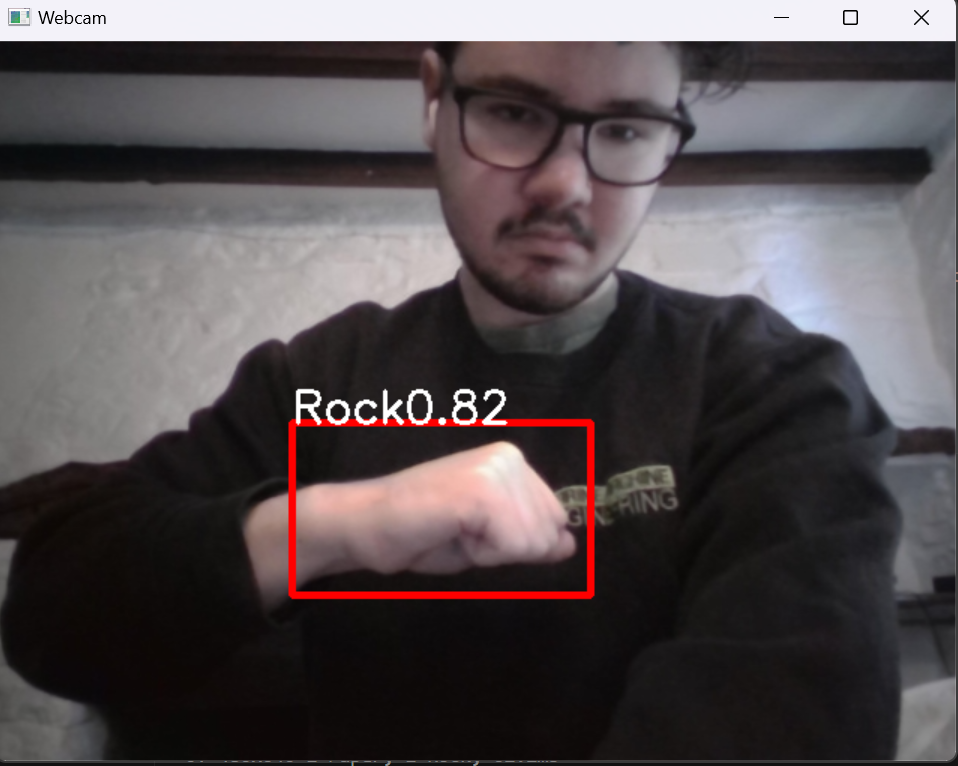
\includegraphics[width=1\linewidth]{method webcam.png}
    \caption{Hand tilt 0 degrees.}
    \label{fig:enter-label}
\end{figure}
\FloatBarrier

After the minute period the average confidence value for the hand gesture was outputted to the terminal to be recorded and plotted on a graph, generated by Excel, for confidence against the angle in a given dimension comparing these two values against each other and seeing the relationship between each hand gesture against these values.

\section{Results}


\begin{figure}[ht]
    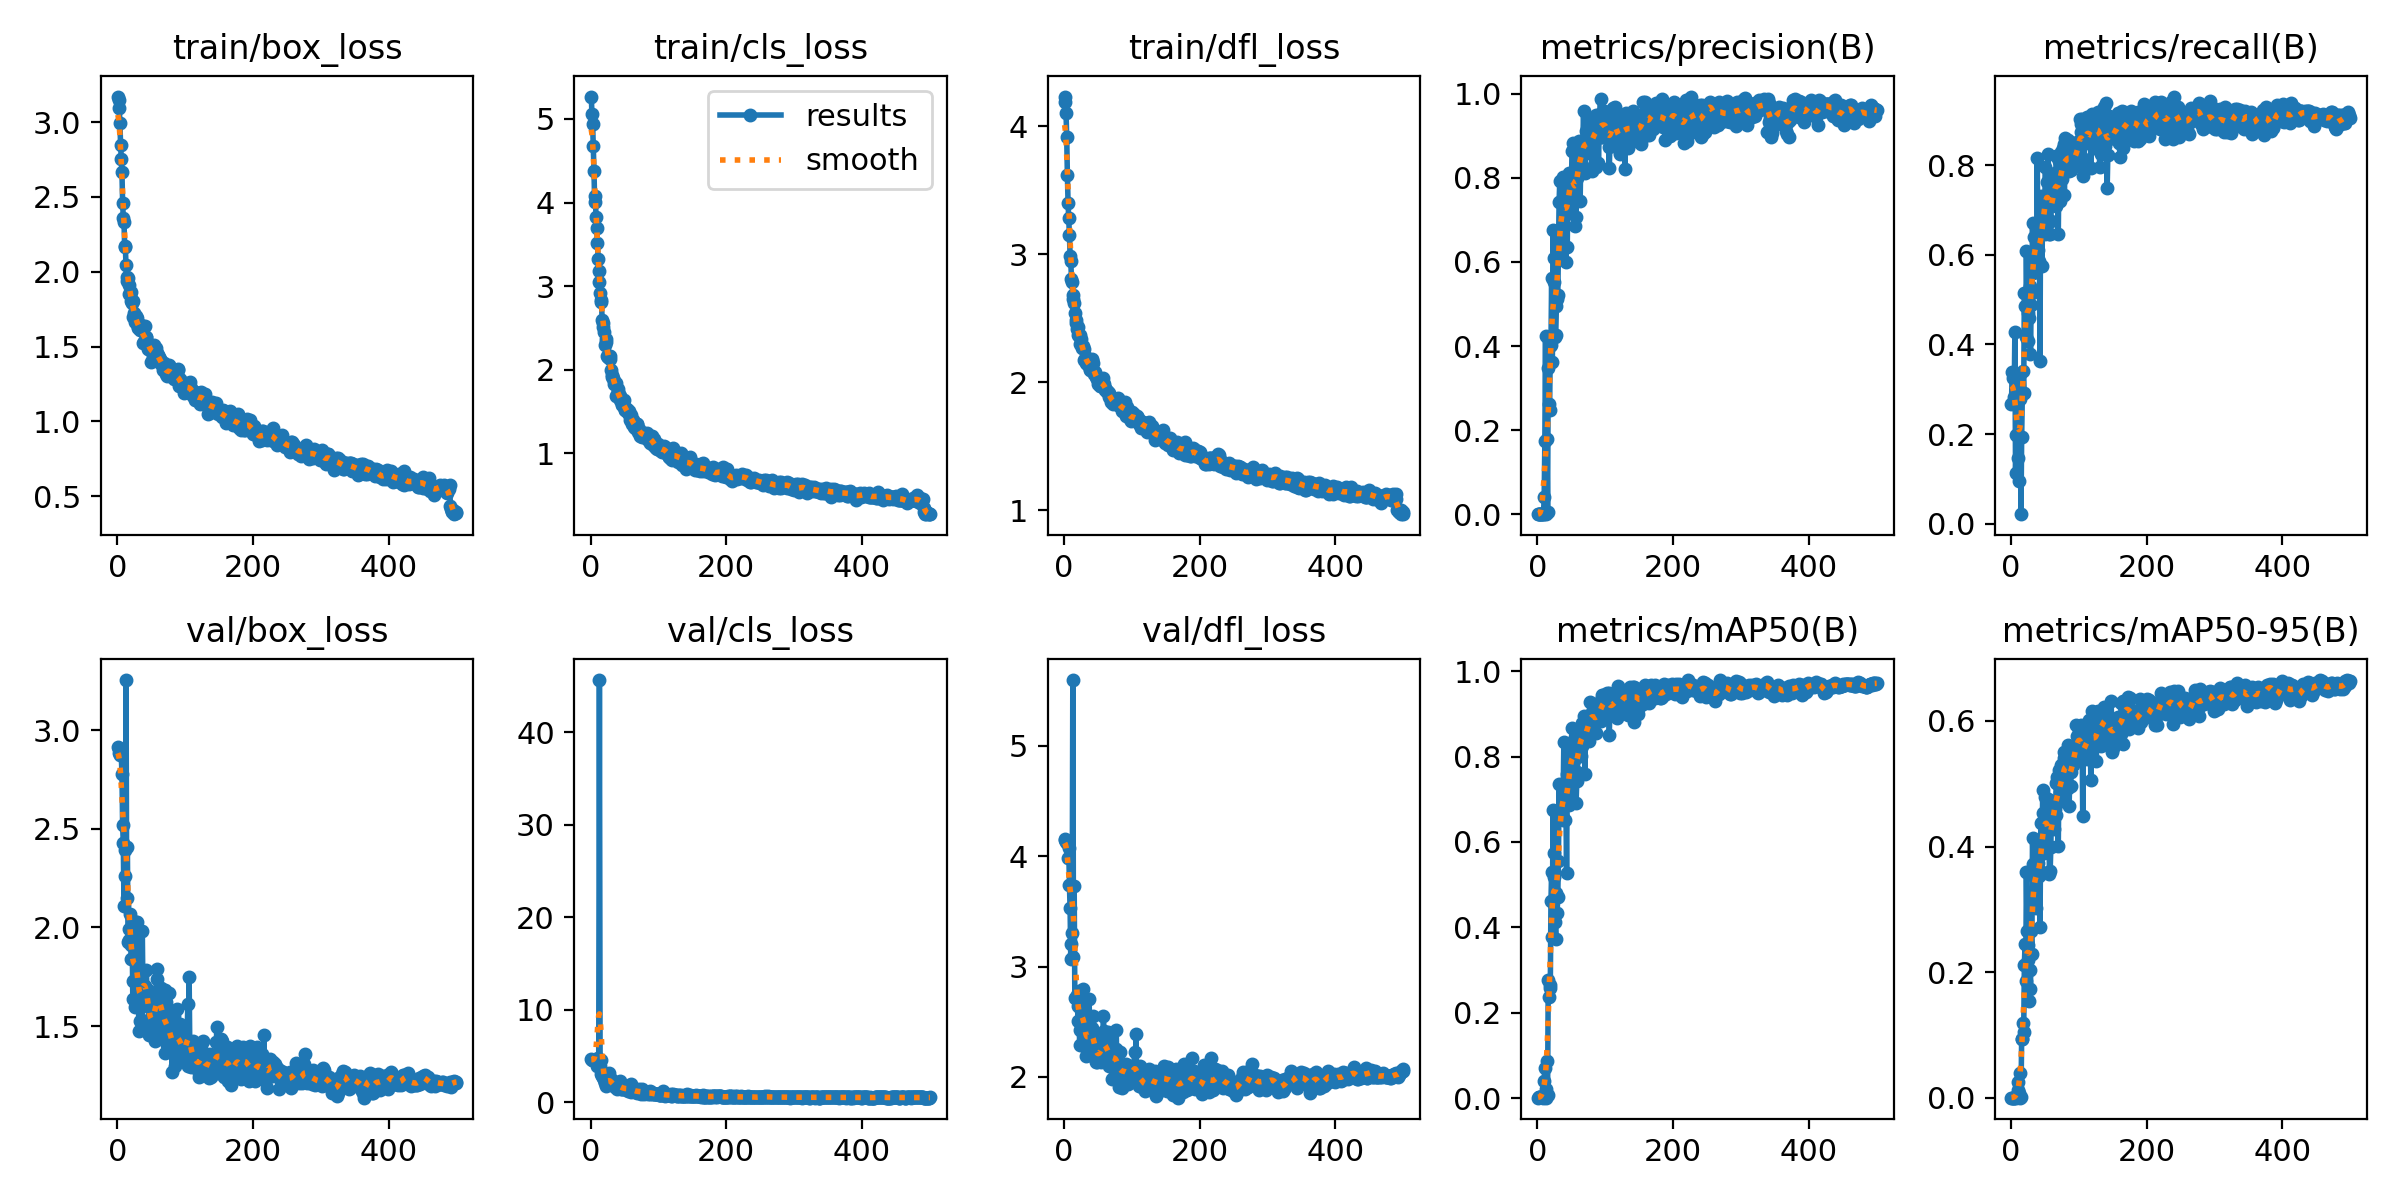
\includegraphics[width=1\linewidth]{results.png}
    \caption{Results for training YOLOv8 AI for 500 Epochs}
    \label{training data}
    In these graphs it can be seen that over the epochs the loss values all decrease but begin to emulate a $e^{-x}.$
    
\end{figure}



\begin{figure}[h]
    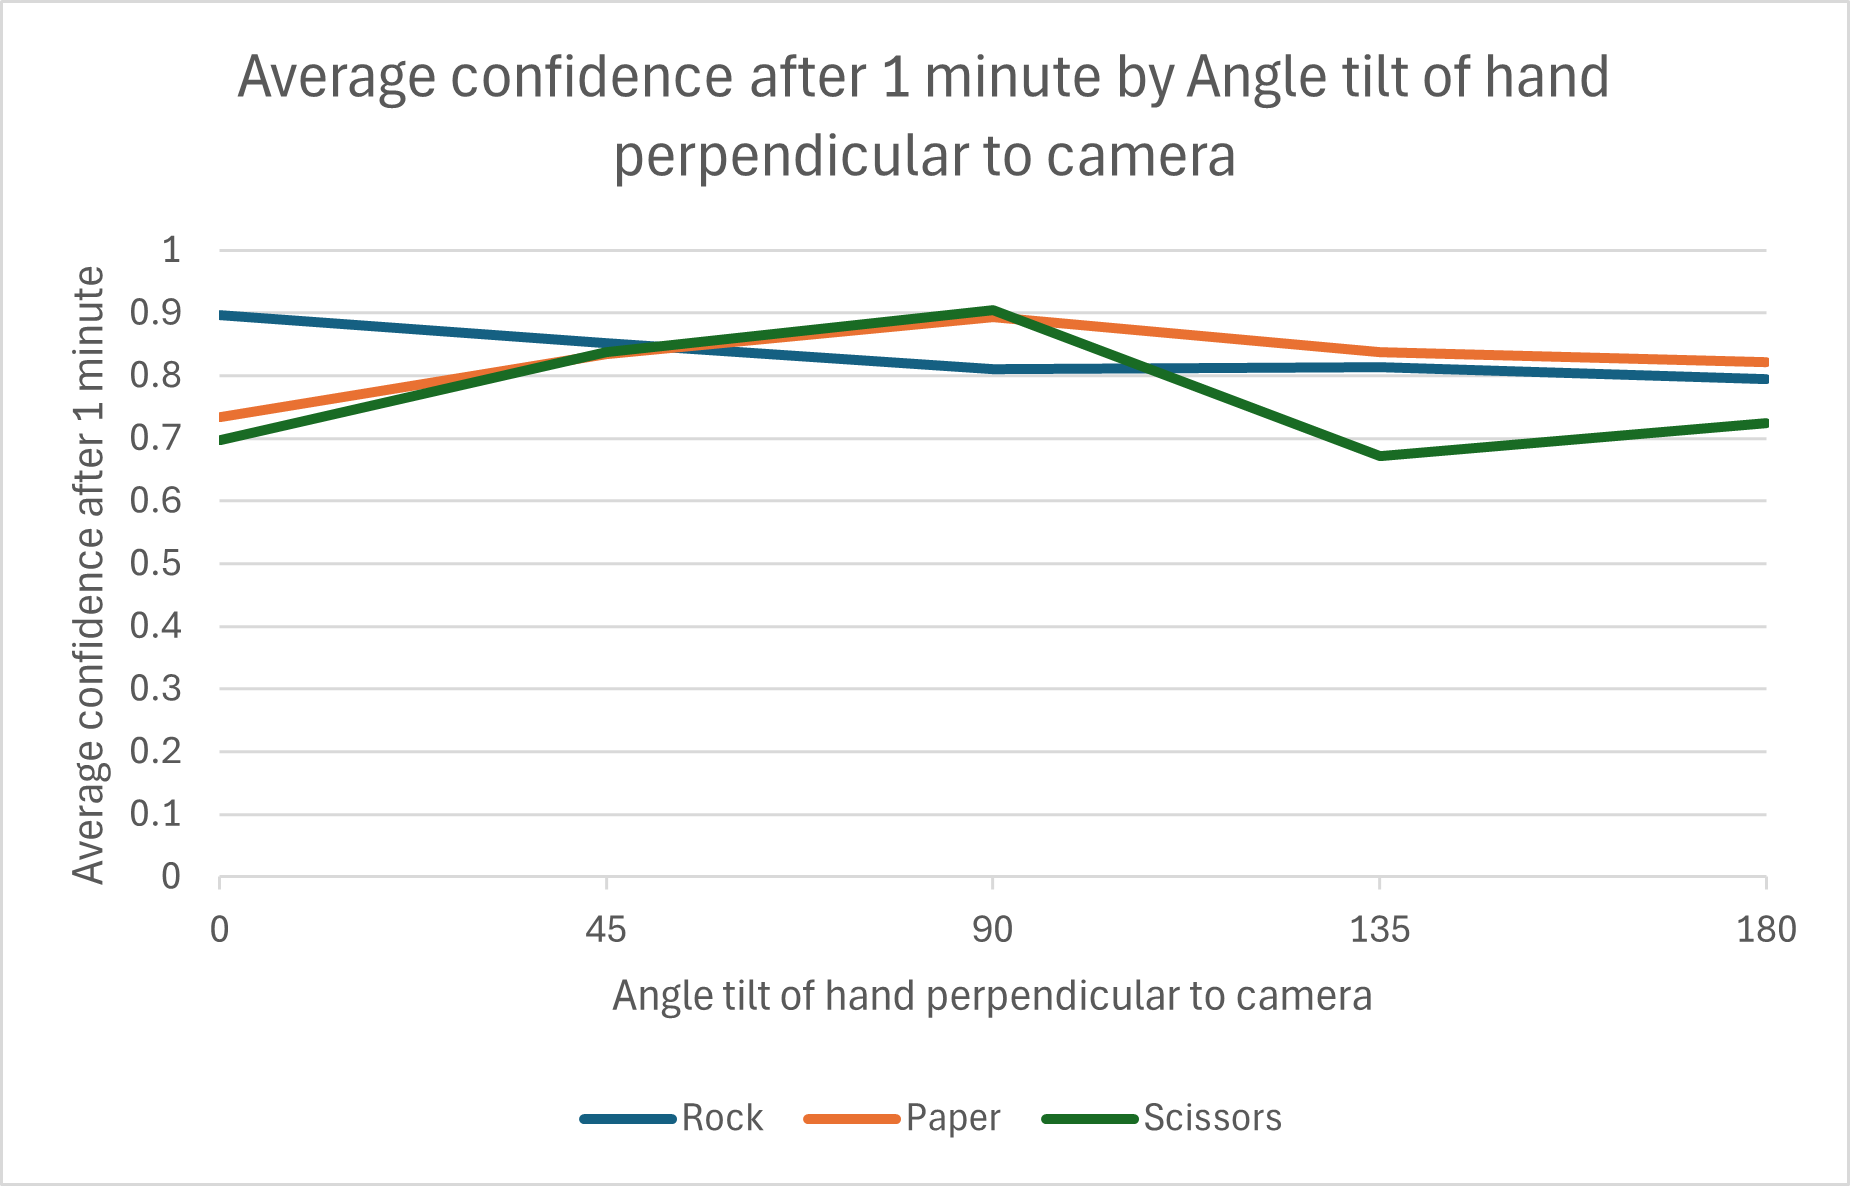
\includegraphics[width=1\linewidth]{Graph for hand tilt.png}
    \caption{Graph for average confidence against hand tilt}
    \label{testing data tilt}

    After 500 epochs the model found that the rock gesture performs best at 0 degrees tilt with an average confidence of 0.897 after 1 minute and the paper and scissors gestures perform best at a 90 degree tilt perpendicular to the camera with an average confidence of 0.893 and 0.905 respectively.
    
\end{figure}
\FloatBarrier



\begin{figure}[h]
    \centering
    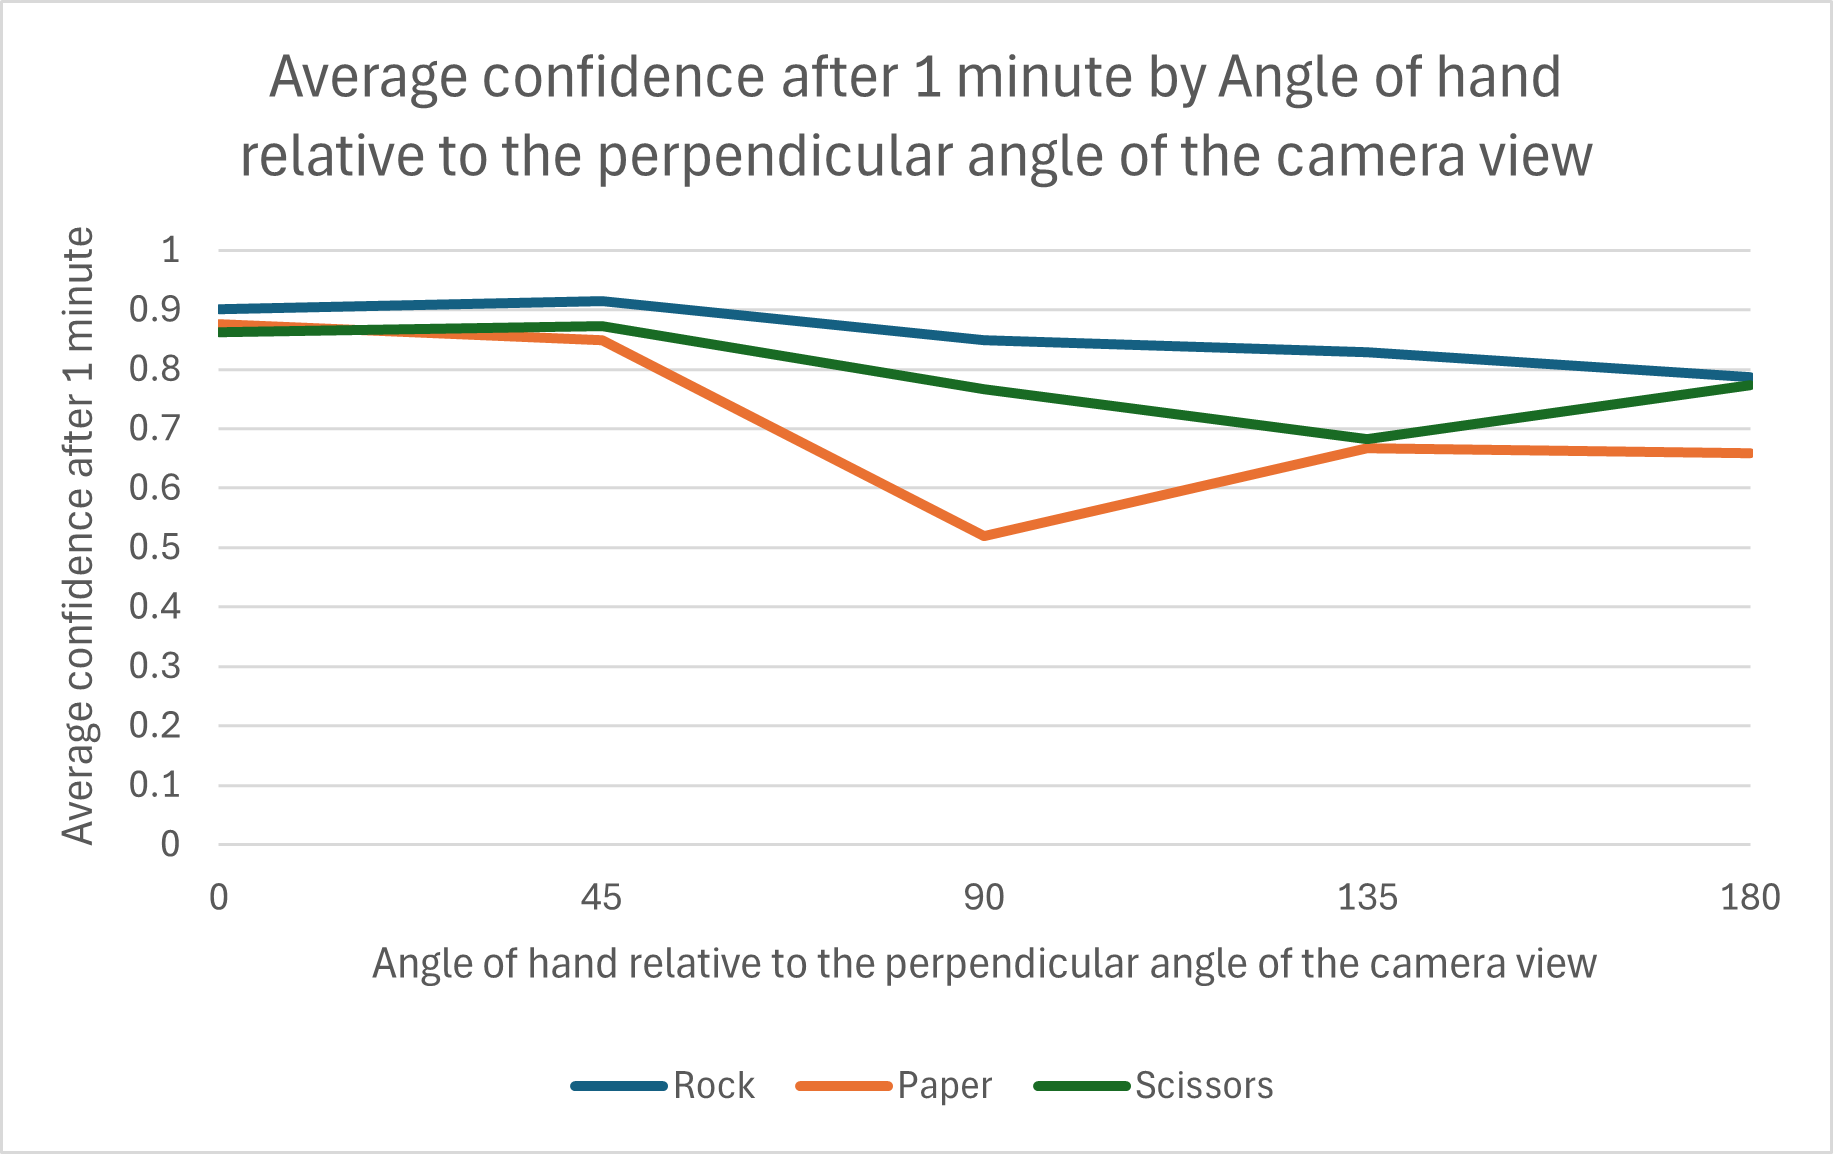
\includegraphics[width=1\linewidth]{Graph for angle of hand relative to perpendicular angle of camera view.png}
    \caption{Graph for angle of hand position}
    \label{testing data position}

    In this graph after 500 epochs it can be seen that the rock and scissors gestures are captured best at a 45 degree angle relative to the perpendicular angle of the camera view with confidence values of 0.914 and 0.873 respectively where as the paper gesture is captured best inline (0 degrees) with the perpendicular angle of the camera view with a confidence value of 0.876.
    
\end{figure}
\FloatBarrier

\section{Analysis}

I believe that the amount of epochs the model was run to was an unsuitable amount and should have been less. You can see from the graphs that as the number of epochs increased the loss value decreases but then begins to become more inconsequential when the number of epochs reached higher than 400. Considering the environmental impact, reducing the amount of epochs for a viable model is positive as it means less GPU usage and less power usage that's being wasted while the future epoch after 400 are not yielding enough benefits in confidence rating.
On reflection the AI technique that was used is very suitable for the problem investigated as it is able to successfully capture the varying hand gestures at different rotations and positions of the hand. However I found that it is more confident with the rock and paper gestures than the scissors, where the slightest change in the distance between the fingers or the thumb position can change the confidence of the model. Furthermore a placement of a hand underneath the gesture, emulating how a classic game of rock, paper, scissors would be played, can increase the confidence at certain angles meaning that more data for more variations in gesture forms and different angles should be added to the dataset to make a more robust system.
While there are techniques out there to help increase the confidence of the system I believe that the technique that I implemented is sufficient if used with a larger dataset encompassing more variations in hand sizes, skin tones and positions to the camera. Whilst this is a game historically in image recognition it can be seen that black people fail to be identified when utilising this software. This is therefore extremely important ethically to create datasets that account for all ethnicities. \cite{algorithmic:racism}


\section{Conclusion}

In conclusion I believe that the implementation of a CNN model through the use of a YOLOv8 library trained on a pre labelled dataset from Roboflow with 825 images was suitable for recognition of hand gestures in a classic game of rock paper scissors yielding good accuracy in most conventional hand positions and tilts with the most reliable gesture for recognition being rock with an overall average confidence value in all positions and tilts of 0.8445.

However the model would benefit from a substantially larger dataset as it can be observed from the testing that when looking at the hand from different angles to the camera's viewpoint both paper and scissors struggled to read with lowest confidence values at 0.658 180 degrees relative to the perpendicular camera view and 0.683 135 degrees respectively. 

Compared to \cite{segmentationRCNN:2018} I believe that the depth data was insignificant in this implementation as the model is only making use of three gestures to recognise and is not required to identify hand gestures at long distance.
I think a beneficial component to add would be the future implementation of SAM \cite{SAM:2023} to segment out the specific hand gesture and remove the background data so that it is unaffected by complex backgrounds.
As I have noted in earlier sections there are environmental sustainability and social and ethical issues relating to the development of an image recognition model that should be taken into account. These include the amount of power used to train the AI model and the variety in ethnicity in a dataset.

In future work I will increase the size of the dataset to account for more variations in hand gestures and shapes using multiple peoples hands with different skin tones, sizes and shapes to provide a more robust algorithm that I will then be able to test the limits of the hand gesture recognition based on factors such as distance from the camera and with complex backgrounds.





\nocite{*} % Insert publications even if they are not cited in the poster
\small{\bibliographystyle{ieeetr}
\bibliography{references}\vspace{0.75in}}

\url{https://github.falmouth.ac.uk/JB261018/COMP213-2102772}


\vspace{12pt}

\end{document}
